%%%%%%%%%%%%%%%%%%%%%%%%%%%%%%%%%%%%%%%%%%%%%%%%%%%%%%%%%%
%
% Vzor pro sazbu kvalifikační práce
%
% Západočeská univerzita v Plzni
% Fakulta aplikovaných věd
% Katedra informatiky a výpočetní techniky
%
% Petr Lobaz, lobaz@kiv.zcu.cz, 2016/03/14
%
%%%%%%%%%%%%%%%%%%%%%%%%%%%%%%%%%%%%%%%%%%%%%%%%%%%%%%%%%%

% Možné jazyky práce: czech, english
% Možné typy práce: BP (bakalářská), DP (diplomová)
\documentclass[czech,BP]{thesiskiv}

% Definujte údaje pro vstupní strany
%
% Jméno a příjmení; kvůli textu prohlášení určete, 
% zda jde o mužské, nebo ženské jméno.
\author{Kateřina Kratochvílová}
\declarationfemale

%alternativa: 
%\declarationfemale

% Název práce
\title{Deskriptor}

% 
% Texty abstraktů (anglicky, česky)
%
\abstracttexten{The text of the abstract (in English). It contains the English translation of the thesis title and a short description of the thesis.}

\abstracttextcz{Text abstraktu (česky). Obsahuje krátkou anotaci (cca 10 řádek) v češtině. Budete ji potřebovat i při vyplňování údajů o bakalářské práci ve STAGu. Český i anglický abstrakt by měly být na stejné stránce a měly by si obsahem co možná nejvíce odpovídat (samozřejmě není možný doslovný překlad!).
}

% Na titulní stranu a do textu prohlášení se automaticky vkládá 
% aktuální rok, resp. datum. Můžete je změnit:
%\titlepageyear{2016}
%\declarationdate{1. března 2016}

% Ve zvláštních případech je možné ovlivnit i ostatní texty:
%
%\university{Západočeská univerzita v Plzni}
%\faculty{Fakulta aplikovaných věd}
%\department{Katedra informatiky a výpočetní techniky}
%\subject{Bakalářská práce}
%\titlepagetown{Plzeň}
%\declarationtown{Plzni}

%%%%%%%%%%%%%%%%%%%%%%%%%%%%%%%%%%%%%%%%%%%%%%%%%%%%%%%%%%
%
% DODATEČNÉ BALÍČKY PRO SAZBU
% Jejich užívání či neužívání záleží na libovůli autora 
% práce
%
%%%%%%%%%%%%%%%%%%%%%%%%%%%%%%%%%%%%%%%%%%%%%%%%%%%%%%%%%%

% Zařadit literaturu do obsahu
\usepackage[nottoc,notlot,notlof]{tocbibind}

% Umožňuje vkládání obrázků
\usepackage[pdftex]{graphicx}

% Odkazy v PDF jsou aktivní; navíc se automaticky vkládá
% balíček 'url', který umožňuje např. dělení slov
% uvnitř URL
\usepackage[pdftex]{hyperref}
\hypersetup{colorlinks=true,
  unicode=true,
  linkcolor=black,
  citecolor=black,
  urlcolor=black,
  bookmarksopen=true}

% matematicke rovnice %
\usepackage{amsmath}

% Při používání citačního stylu csplainnatkiv
% (odvozen z csplainnat, http://repo.or.cz/w/csplainnat.git)
% lze snadno modifikovat vzhled citací v textu
\usepackage[numbers,sort&compress]{natbib}

%%%%%%%%%%%%%%%%%%%%%%%%%%%%%%%%%%%%%%%%%%%%%%%%%%%%%%%%%%
%
% VLASTNÍ TEXT PRÁCE
%
%%%%%%%%%%%%%%%%%%%%%%%%%%%%%%%%%%%%%%%%%%%%%%%%%%%%%%%%%%
\begin{document}
%
\maketitle
\tableofcontents


\chapter{Zadání}
Vytvořit deskriptor pro detekci hran u barevných obrázků.


\section{Výpočet gradientu}
POEM deskritpro se používá jen na šedoonový obrázek, my by jsme ho chtěli na barevný obrázek
\subsection{Vyýpočet u šedotónového obrázku}

\subsection{Výpočet}
Nejprve je potřeba vypočítát gradient. Gradeint je směr růstu. Podle některých studii jsou nejlepší jednoduché masky jako je např. $[1, 0, -1]$ a $[1, 0, -1]^T$. Okraje se buď vypouštějí nebo se dají doplnit (existuje více způsobů doplňění). Masky použijeme na obrázek a vypadnou nám obrázky o rozměrech mxn každý bod původního obrázku je reprezentován jako 2D vektor. Pokud si vektor rozložíme na x a y složku dostali bychom dva obrázky jeden, který reprezentuje obrázek po použití x-ového filtru, a druhý který reprezentuje obrázek po použití y-filtru. Přičemž použití  y filtru by nám mělo zvíraznit hrany v ylonovém směru (svislé) a x zvírazní hrany v x směru (vodorovné).

TODO doplnit obrázky gradient 

Magnituda\\
Magnituda je velikost směru růstu lze si ji představit jako velikost směru růstu pro každý pixel. Počítá se pro každý pixel. Takže se dá počítat jako velikost těch 2D vektrů které jsme dostaly při výpočtu gradientu.
Magnituda představuje velikost vektoru gradientu.
Velikost vektoru v rovině:
\begin{align}
   \label{velikost_vektoru} |u| = \sqrt{u_1^2 + u_2^2}
\end{align}



\section{Textura}
LBP i Gabor pracují s informací o intenzitě obrazu. Detekce hran. Obyčejné LBP problém s rotací.


kombinace textur a barevne informace
1. Vytvoření společného příznaku, 
například rozšíření LBP na všechny barvené kanály
informace o barvě a textuře se mohou oblivňovat protichůdně

2. Vyhodnotit a klasifikovat příznaky odděleně a pak výslednou klasifikaci nějak s pojit z několika částí 
	to je například JEC
	
	výhoda zachovává vlastnosti obou původních příznaků 
	výpočetně náročnější a jeho úspěšnost je přímo závislá na způsobu kombinace obou informací	
	
vutbrno 117319 10 stranka




Gabor filter je lineární filter používaný pro detekci hran. Frekvence a orientace reprezentující Gabor filter je podobná lidskému vnímání a jsou zvláště vhodné pro reprezentaci textury a rozlišování. 

Gabor filtr reaguje na hrany a texturové změny. 

Obrázky jsou filtrovány za použité reálné části z různých odlišních Gabor filtrů jader. Průměrný a rozptyl filtrovaných snímků jsou pak použity jako funkce pro klasifikaci, která je založena na nejméně kvadratické chyby pro jednoduchost.


TODO Dohledat Haar a Gabor wavelety, přidat vzorečky a zase klidně i obrázky

\subsection{Barva}
U digitálního obrazu je barva reprezentovaná n-rozměrným vektorem. Jeho velikost a význam jednotlivých složek (tzv. barevných kanálů) zavisí na příslušném barevném prostoru. Počet bitů použitých k uložení buď celého vektoru nebo jeho jednotlivých složek se nazývá barevná hloubka (totožně bitová hloubka). Obvykle se můžeme setkat s hodnotami 8, 12, 14 a 16 bitů na kanál. 
\\
V použité metodě získáme vlastnosti z obrázků ve třech rozdílných barevných prostorech: RGB, HSV a LAB. RGB (Red, Green, Blue) je nejobvykleji používaný pro zachycení obrázu nebo jeho zobrazení. Oproti tomu HSV (Hue, Saturation and Value) se snaží zachytit barevný model tak jak ho vnímá lidské oko, ale zároveň se snaží zůstat jednoduchý na výpočet. Hue znamená odstín barvy, saturation systost barvy a value je hodnota jasu nebo také množství bílého světla. RGB je závislý na konkrétním zařízení, nemůže dosáhnout celého rozsahu barev, které vidí lidské oko, zatímco barevný model LAB je shopen obsáhnout celé viditelné spektrum a navíc je nezávislý na zařízení. L (ve zkratce LAB) značí Luminanci (jas dosahuje hodnot 0 - 100, kde 0 je černá a 100 je bílá). Zbylé A a B jsou dvě barvonosné složky, kdy A je ve směru červeno/zeleném a B se pohybuje ve směru modro/žlutém. 


Pro RGB, HSV i LAB použijeme barevnou hloubku 16 bitů na kanál histogramu v jejich příslušném barevném prostoru. 

Jako reprezentace textur budou použity Gabor a Haar wavelety. Každý obrázek bude filtrován s Gabor wavelet na třech škálách a čtyřech orientacích. 








\begin{figure}[h]
		\centering
		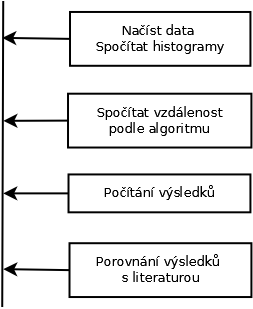
\includegraphics[width=253px]{./img/graf.png}	
		\caption{Návrh systému}
\end{figure}


\chapter{Použité programové prostředky}
Program byl navržen na operační systému Linux. Jako programovací jazyk byl zvolen Python a to z důvodu jeho jednoduchého použití, což je na prototyp, jako je tento velice výhodné na časovou náročnost. Program využívá knihovnu OpenCV 3.1. 
  
\section{OpenCV}
OpenCV (Open source computer vision) je knihovna vydávána pod licencí BSD a je volně k dispozici jak pro akademické účely, tak pro komerční použití. Je vhodná pro použití v C++, C, Python a Javě. Podporuje operační systémy Windows, Linux, Mac OS, iOS a Android.
\\
Knihovna byla navrhnuta pro výpočetní efektivitu v oblasti počítačového vidění a zpracování obrazu se zaměřením na zpracování obrazu v reálném čase. Z důvodu optimalizace byla napsána v C/C++. 
\\
Knihovnu OpenCV je možné stáhnout na adrese: http://opencv.org/


\chapter{Závěr}
V teoretické části byly popsány nízkoúrovňové příznaky barva a textura. Byla rozebrána metoda JEC, která bude v bakalářské práci implementována. Seznámili jsme se s knihovnou OpenCV, prostudovali obrázky a přiložená metadata od ČTK, ESP a iaprtc12. 

\chapter{Uživatelská dokumentace}
popsani jak vypada zdrojovej soubor kterej to zere, nejdriv cesta k souboru a pak jeho klicovy slova
 
% 
% PRO ANGLICKOU SAZBU JE NUTNÉ ZMĚNIT
% CITAČNÍ STYL!
%
\bibliographystyle{csplainnatkiv}
{\raggedright\small
\bibliography{literatura}
}

\end{document}
